% Copyright 2004 by Till Tantau <tantau@users.sourceforge.net>.
%
% In principle, this file can be redistributed and/or modified under
% the terms of the GNU Public License, version 2.
%
% However, this file is supposed to be a template to be modified
% for your own needs. For this reason, if you use this file as a
% template and not specifically distribute it as part of a another
% package/program, I grant the extra permission to freely copy and
% modify this file as you see fit and even to delete this copyright
% notice. 
  
\documentclass[spanish,pdf]{beamer}
\usepackage[spanish,es-tabla]{babel}
\usepackage[utf8]{inputenc}
\usepackage{amsmath,amssymb,latexsym}
% Doe's not play well with memoir
\usepackage{subfigure}
%\usepackage{pifont}
%\usepackage[linktocpage=true]{hyperref}
%\usepackage{MnSymbol}
%\usepackage{algorithm}
%\usepackage[noend]{algpseudocode}
\usepackage{wrapfig}
\usepackage{xspace}
\usepackage{multirow}
\usepackage{adjustbox}
\usepackage[figuresleft]{rotating}
\usepackage{rotfloat}
\usepackage[final]{fixme}
\usepackage{multicol}
\usepackage{tikz}
\usetikzlibrary{automata,petri,positioning,shapes,snakes,arrows,backgrounds,babel}
\tikzstyle{tplace}=[circle,draw,inner sep=1.8mm]
\usepackage{amsthm}
% Encabezado "lindo"
% Memoir y fancyhdr definen ambos esto. Pero lo definen igual, así que no hay problema
% Fuente: http://tex.stackexchange.com/questions/37868/fancyhdr-and-memoir
\let\footruleskip\undefined
\usepackage{fancyhdr}
% Saca los espacios adicionales de las listas tipo itemize
%\usepackage{enumitem}
%\setlist{nolistsep}
%\usepackage{hypcap}
% Para armar código bonito
%\usepackage{minted}
%\usemintedstyle{bw}
\usepackage{xcolor}
\usepackage[framemethod=default]{mdframed}
\definecolor{bg}{rgb}{0.95,0.95,0.95}
\mdfdefinestyle{codebox}{backgroundcolor=bg,skipabove=10,linewidth=0}
\usepackage[most]{tcolorbox}

\usepackage{czt}
\usepackage{algpseudocode}
\setbeamerfont{block body}{size=\scriptsize}
%\usepackage{xcolor}
%
%\usepackage[most]{tcolorbox}

%\usetheme{Madrid}
%\usetheme{Antibes}
%\usetheme{Copenhagen}
\usetheme{Warsaw}
\mode<presentation>{} 

\newcommand{\til}{\widetilde}
%\newcommand{\inv}{\overline}
\newcommand{\bsl}{\backslash}
\newcommand{\loor}{\vee}
\newcommand{\loand}{\wedge}
\newcommand{\xor}{\oplus}
\newcommand{\subs}{\subset}
\newcommand{\subse}{\subseteq}
\newcommand{\sups}{\supset}
\newcommand{\supse}{\supseteq}
\newcommand{\ror}{\vdash}
\newcommand{\Ror}{\models}
\newcommand{\rar}{\rightarrow}
\newcommand{\mrar}{$\rightarrow$}
\newcommand{\Rar}{\Rightarrow}
\newcommand{\URar}[1]{\stackrel{#1}{\Rar }}
\newcommand{\Urar}[1]{\stackrel{#1}{\rar }}
\newcommand{\ULRar}[1]{\stackrel{#1}{\Longrightarrow }}
\newcommand{\Ulrar}[1]{\stackrel{#1}{\longrightarrow }}
\newcommand{\paral}{\parallel}
\newcommand{\emptys}{\emptyset}
\newcommand{\mult}{\times}
\newcommand{\verx}{\vspace{12pt}}
\newcommand{\niz}{\vspace{10pt}}
\newcommand{\eproof}{\hspace{\fill} $\Box $}
\newcommand{\ediamon}{\hspace{\fill} $\Diamond $}


% Alex's predicates

\newcommand{\ins}{\mbox{\tt in}}
\newcommand{\IN}{\mbox{\tt IN}}
\newcommand{\out}{\mbox{\tt out}}
\newcommand{\OUT}{\mbox{\tt OUT}}
\newcommand{\INOUT}{\mbox{\tt IN\_OUT}}
\newcommand{\exit}{\mbox{\tt exit}}
\newcommand{\EXIT}{\mbox{\tt EXIT}}
\newcommand{\enter}{\mbox{\tt enter}}
\newcommand{\nocross}{\mbox{\tt nocross}}
\newcommand{\ENTER}{\mbox{\tt ENTER}}
\newcommand{\inexit}{\mbox{\tt in\_exit}}
\newcommand{\inenter}{\mbox{\tt in\_enter}}
\newcommand{\enterexit}{\mbox{\tt enter\_exit}}
\newcommand{\exitenter}{\mbox{\tt enter\_exit}}
\newcommand{\outexit}{\mbox{\tt out\_exit}}
\newcommand{\outenter}{\mbox{\tt out\_enter}}
\newcommand{\genet}{\mbox{\tt Genet}}
\newcommand{\petrify}{\mbox{\tt petrify}}
\newcommand{\mlc}{\mbox{\tt MLC}}

\newtheorem{exam}{Example}[section]
\newtheorem{prop}{Proposition}[section]
\newenvironment{condition}[1]{\noindent{\bf Condition #1.} \em}{\rm \\}

\newcommand{\bop}{\noindent{\bf Proof: }}
\newcommand{\eop}{$\square$ \\}
%\newenvironment{proof}{\bop}{\eop}
%\newtheorem{lemma}{Lemma}[section]
%\newtheorem{theorem}{Theorem}[section]
%\newtheorem{corollary}{Corollary}[section]
%\newtheorem{proposition}{Proposition}[section]
%\newtheorem{property}{Property}[section]
%\newtheorem{definition}{Definition}[section]
%\newtheorem{problem}{Problem}[section]
%\newtheorem{procedure}{Procedure}[section]
%\newtheorem{restriction}{Restriction}[section]
%\newtheorem{algorithm}{Algorithm}
\def\acs/{{\sf ACS}}
\def\ets/{{\sf ETS}}
\def\ec/{{\sf EC}}
\def\eec/{{\sf EEC}}
\def\ects/{{\sf ECTS}}
\def\eects/{{\sf EECTS}}
\def\nts/{{\sf NTS}}
\def\gnts/{{\sf GNTS}}
\def\eer/{{\sf EER}}
\def\esr/{{\sf ESR}}
\def\en/{{\sf EN}}
\def\ger/{{\sf GER}}
\def\er/{{\sf ER}}
\def\sr/{{\sf SR}}
\def\gsr/{{\sf GSR}}
\def\bacs/{{\sf BACS}}
\def\ts/{{\sf TS}}
\def\lts/{{\sf LTS}}
\def\alts/{{\sf ALTS}}
\def\std/{{\sf STD}}
\def\cd/{{\sf CD}}
\def\alc/{{\sf ALC}}
\def\id/{{\sf ID}}
\def\pd/{{\sf PD}}

\def\stg/{{\sf STG}}
\def\cln/{{\sf CLN}}
\def\clstg/{{\sf CL-STG}}
\def\btm/{{Binary Trace Model}}
\def\tm/{{Trace Model}}

\newcommand{\pn}{\textsf{PN}}
\newcommand{\rg}{\textsf{RG}}
\newcommand{\rs}{\textsf{RS}}
\newcommand{\prs}{\textsf{PRS}}
\newcommand{\pl}{\textsf{PL}}

\newcommand{\mg}{\mbox{\textsf{MG}}}       % Marked graph
\def\dr/{{Distributive}}
\def\drone/{{Distributive-1}}
\def\drtwo/{{Distributive-2}}
\def\op/{{Output-persistent}}
\def\sm/{{\sf SM}}
\def\bull{\vrule height .9ex width .8ex depth -.1ex }
%\def\trans#1{\stackrel{#1}{\rightarrow}}
\def\dquote#1{``#1''}
\def\trans#1{[#1>}
\def\etrans#1{E(#1)}
\def\vect#1#2{$#1_1,\ldots,#1_{#2}$}
\def\assign#1#2{\mbox{$#1 \leftarrow #2$}}
\def\tild{{\verb+~+}}
\def\pred#1{\,^\bullet #1}
\def\succ#1{#1^\bullet}
\def\prereg#1{\,^\circ #1}
\def\postreg#1{#1^\circ}
\def\prepostreg#1{\,^\circ #1^\circ}
\def\endofproof{\hspace{\fill} $\Box $}


\def\grad#1#2{\Delta_{#1}(#2)}
\def\pow#1{#1^\diamond}
\def\enabling#1{^\star#1}
\def\rzero{\mbox{\bf 0}}
\def\rone{\mbox{\bf 1}}
\def\rk{\mbox{\bf K}}
\def\REG{{\mathcal R}}
\def\TOP{\sqcap}
\def\sup{\mbox{\em supp}}
\def\topk{\top}
%  Nomenclature for Petri nets, STGs, etc.

\newcommand{\reachm}[1]{[#1\rangle}             % reachable markings
\newcommand{\firing}[3]{\mbox{$#1\Ulrar{#2} #3$}} % Transition firing
\newcommand{\altfiring}[3]{#1[#2\rangle #3}        % Alternative transition firing
\newcommand{\preset}[1]{\mbox{$^\bullet#1$}}             % Preset
\newcommand{\postset}[1]{\mbox{$#1^\bullet$}}            % Postset
\newcommand{\pmlog}{\ensuremath{{\mathcal L}}}        % Log
\newcommand{\pmlogp}{\ensuremath{{\mathcal L}}\textsuperscript{+}}        % Positive Log
\newcommand{\pmlogn}{\ensuremath{{\mathcal L}}\textsubscript{-}}        % Negative Log
\newcommand{\ph}{\ensuremath{{\mathcal P}}}          % Polyhedron
\newcommand{\parikh}[1]{\ensuremath{\Pi(#1)}}    % Set of Parikh vectors

% Natural numbers
%\newcommand{\nat}{\ensuremath{\mathbb{N}}}

\newcommand\bench[2][]{%
\if\relax\detokenize{#1}\relax%
\textsc{#2}\else \textsc{#2}\hspace{0.3pt}{\footnotesize(}#1{\footnotesize)}\fi\@\xspace}

\newcommand\pnsimp  {\textsc{PNsimpl}\@\xspace}
\newcommand\pachtool  {\textsc{PacH}\@\xspace}
\newcommand\qhulltool  {\textsc{Qhull}\@\xspace}

\newcommand{\model}{\mathcal{M}}
\newcommand{\sys}{\mathcal{S}}
\newcommand{\Language} {\mathcal{L}}


\newcommand{\nlgtext}[1] {``\emph{#1}''}
\newcommand{\nlgfun}[1] {\texttt{#1}}
\newcommand{\reglaverb}[2]{\item #1 \\ \hspace*{0.56cm} $\rightarrow$ #2}
% fix para 
\renewcommand*\Call[2]{\textproc{#1}(#2)}

% Equations commands
% Begin equation no numbered
\newcommand{\bnnequation}{\begin{equation*}}
% Begin equation mode
\newcommand{\bequation}{\begin{equation*}}
% Begin equation mode with label
\newcommand{\bequationl}[1]{\begin{equation}\label{eq:#1}}
% End equation mode
\newcommand{\eequation}{\end{equation*}}
% End labeled equation mode
\newcommand{\eequationl}{\end{equation}}
% End equation no numbered
\newcommand{\ennequation}{\end{equation*}}

%Math symbols
\newcommand{\sigmap}{\ensuremath{\sigma}\textsuperscript{+}}        % Positive Sigma
\newcommand{\sigman}{\ensuremath{\sigma}\textsuperscript{-}}        % Negative Sigma
\newcommand{\eventstar}{\ensuremath{T}\textsuperscript{*}}        % Event Set T*

% Condensed table
\newcommand\newrow{\\[-1.5pt]}
\newcommand\tvdots{\multicolumn{1}{c}{$\vdots$}}

% Scale input
\newcommand{\scaledinput}[2]{\scalebox{#1}{\input{#2}}}


\definecolor{mygreen}{rgb}{0,0.5,0}
% Algoritmos en español
\floatname{algorithm}{Algoritmo}
%\renewcommand{\listalgorithmname}{Lista de algoritmos}
\renewcommand{\algorithmicrequire}{\textbf{Entrada:}}
\renewcommand{\algorithmicensure}{\textbf{Salida:}}


\AtBeginSection[]
{
  \begin{frame}<beamer>
    \frametitle{Contenidos}
    \tableofcontents[currentsection]
  \end{frame}
}
  
%\title{Generación de lenguaje natural a partir de clases de prueba del \textit{test template framework}}
  
% A subtitle is optional and this may be deleted
%\subtitle{Optional Subtitle}
  
%\author{F.~Author\inst{1} \and S.~Another\inst{2}}
% - Give the names in the same order as the appear in the paper.
% - Use the \inst{?} command only if the authors have different
%   affiliation.
  
%\institute[Universities of Somewhere and Elsewhere] % (optional, but mostly needed)
%{
%  \inst{1}%
%  Department of Computer Science\\
%  University of Somewhere
%  \and
%  \inst{2}%
%  Department of Theoretical Philosophy\\
%  University of Elsewhere}
% - Use the \inst command only if there are several affiliations.
% - Keep it simple, no one is interested in your street address.
  
%\date{Conference Name, 2013}
% - Either use conference name or its abbreviation.
% - Not really informative to the audience, more for people (including
%   yourself) who are reading the slides online
  
\subject{Computer Science}
% This is only inserted into the PDF information catalog. Can be left
% out. 
  
% If you have a file called "university-logo-filename.xxx", where xxx
% is a graphic format that can be processed by latex or pdflatex,
% resp., then you can add a logo as follows:
  
\pgfdeclareimage[height=0.5cm]{university-logo}{../img/unr.png}
\logo{\pgfuseimage{university-logo}}
  
% Delete this, if you do not want the table of contents to pop up at
% the beginning of each subsection:
%\AtBeginSubsection[]
%{
%    \begin{frame}<beamer>{Contenidos}
%        \tableofcontents[currentsection,currentsubsection]
%    \end{frame}
%}
  
% Let's get started
\begin{document}
  
\title[Generación y simplificación de especificaciones de procesos]{Generación y simplificación automática de especificaciones de procesos}
\institute[FCEIA - UNR]{
  Departamento de Ciencias de la Computación\\
  Facultad de Ciencias Exactas, Ingeniería y Agrimensura\\
  Universidad Nacional de Rosario
}
\author[Lucio Nardelli]{\begin{tabular}{r@{ }l} 
  Autor:      & Lucio Nardelli \\[1ex]
  Director:   & Hernán Ponce de León\\
  \end{tabular}}
\date{Junio, 2016}
  
\begin{frame}
  \titlepage
\end{frame}
  
%\begin{frame}{Outline}
  %\tableofcontents
  % You might wish to add the option [pausesections]
%\end{frame}
  
\section{Introducción}
  
\begin{frame}{Motivación}{}
    \begin{itemize}
      \setlength\itemsep{0.4cm}
      \item<2-> Hoy en día existe un acceso masivo a sistemas informáticos.
      \item<3-> Esto genera inmensas cantidades de información.
      \item<4-> Existe una dependencia total de estos sistemas por lo que es
                esencial mantenerlos eficientes y seguros.
      \item<5-> ¿Cómo se puede asegurar esto?
      \item<6-> Para esto utilizaremos métodos de representación formal.
    \end{itemize}
\end{frame}

\begin{frame}{Motivación}{Modelos formales}
  \vspace*{-0.5cm}
  \begin{minipage}[c][0.4\textheight][c]{\linewidth}
    Contar con un modelo claro y simple permite una mejor comprensión del sistema 
    subyacente y posibilita además, aplicar diferentes métodos de optimización
    del flujo general del sistema.
  \end{minipage}
  \begin{columns}
    \column{0.25\textwidth}
  \pause 
      \begin{minipage}[c][0.3\textheight][c]{\linewidth}
        \centering
        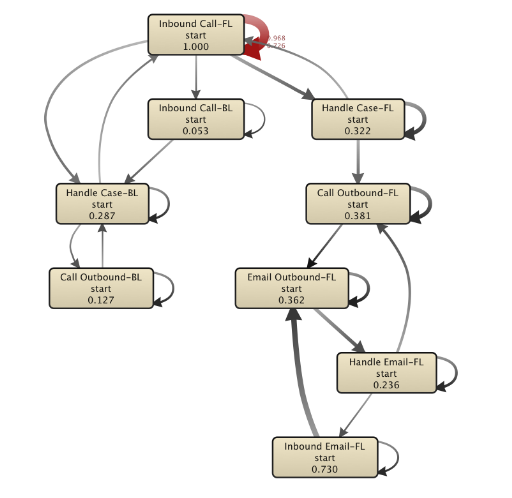
\includegraphics[width=1.2\linewidth]{img/ejemplo1.png}
      \end{minipage}
    \column{0.45\textwidth}
  \pause 
      \begin{minipage}[c][0.3\textheight][c]{\linewidth}
        \centering
        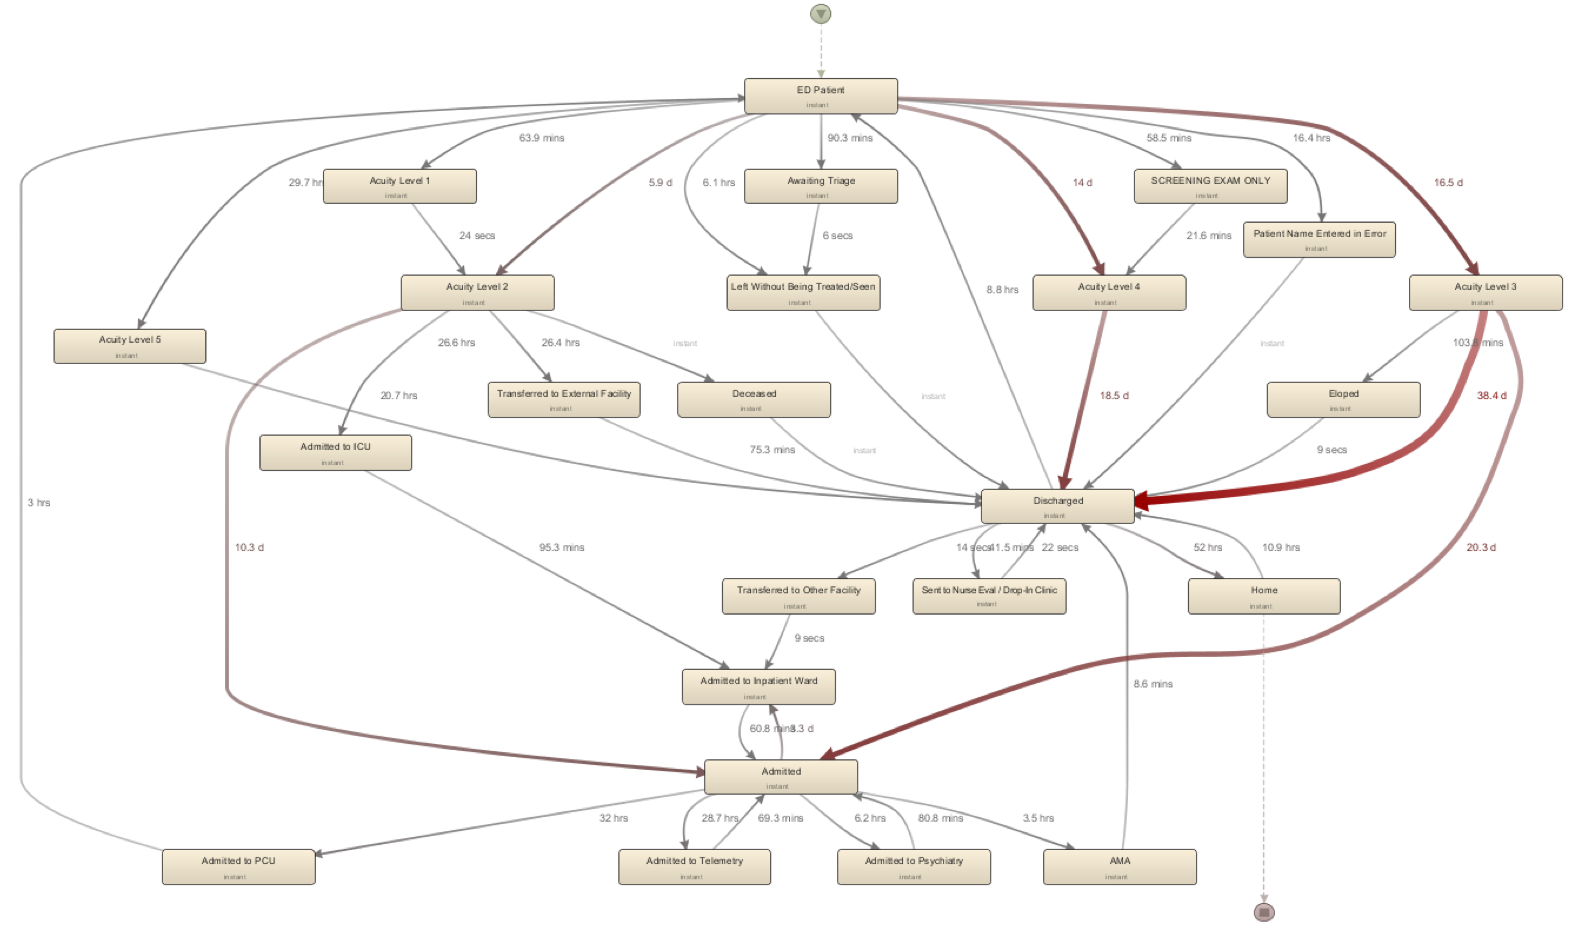
\includegraphics[width=1.2\linewidth]{img/ejemplo2.png}
      \end{minipage}
    \column{0.3\textwidth}
  \pause 
      \begin{minipage}[c][0.05\textheight][c]{\linewidth}
        \centering
        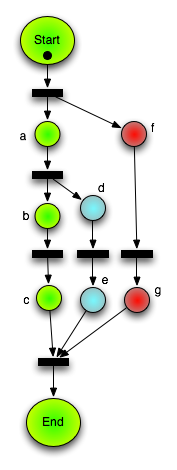
\includegraphics[width=0.5\linewidth]{img/ejemplo3.png}
      \end{minipage}
  \end{columns}
  \vspace*{-0.5cm}
  \pause 
  \begin{minipage}[c][0.4\textheight][c]{\linewidth}
    El problema es que estos modelos formales, ¡rara vez existen!
  \end{minipage}
\end{frame}

\begin{frame}{Motivación}{Descubrimiento de procesos}
    \begin{itemize}
      \setlength\itemsep{0.4cm}
      \item<2-> Para resolver este inconveniente recurrimos a una de las áreas de la
                minería de procesos: el \textit{descubrimiento de procesos}.
      \item<3-> El descubrimiento de procesos consiste en una técnica de aprendizaje automatizado
                que permite obtener un modelo formal a partir de los registros de las acciones
                relevantes que ocurren durante la ejecución de un sistema.
                
                %los \textit{logs de eventos} de un sistema.
    \end{itemize}
%    \pause[4]
%        Pero...¿qué es un log de eventos de un sistema?
%    \begin{itemize}
%      \item<5-> Un log de eventos consiste de un archivo donde se describe un conjunto de trazas de un sistema; 
%          es decir se lleva registro ordenado de las acciones relevantes que ocurren durante la ejecución de un sistema.
%    \end{itemize}
\end{frame}

%\begin{frame}{Motivación}{Mejora de modelos}
%    \begin{itemize}
%      \setlength\itemsep{0.4cm}
%      \item<2-> El problema con las técnicas de descubrimiento es que, en ocasiones, generan modelos
%                demasiado complejos, conocidos como modelos \textit{spaghetti}.
%      \end{itemize}
%      \pause[3]
%      \begin{columns}
%        \column{0.5\textwidth}
%          \centering
%          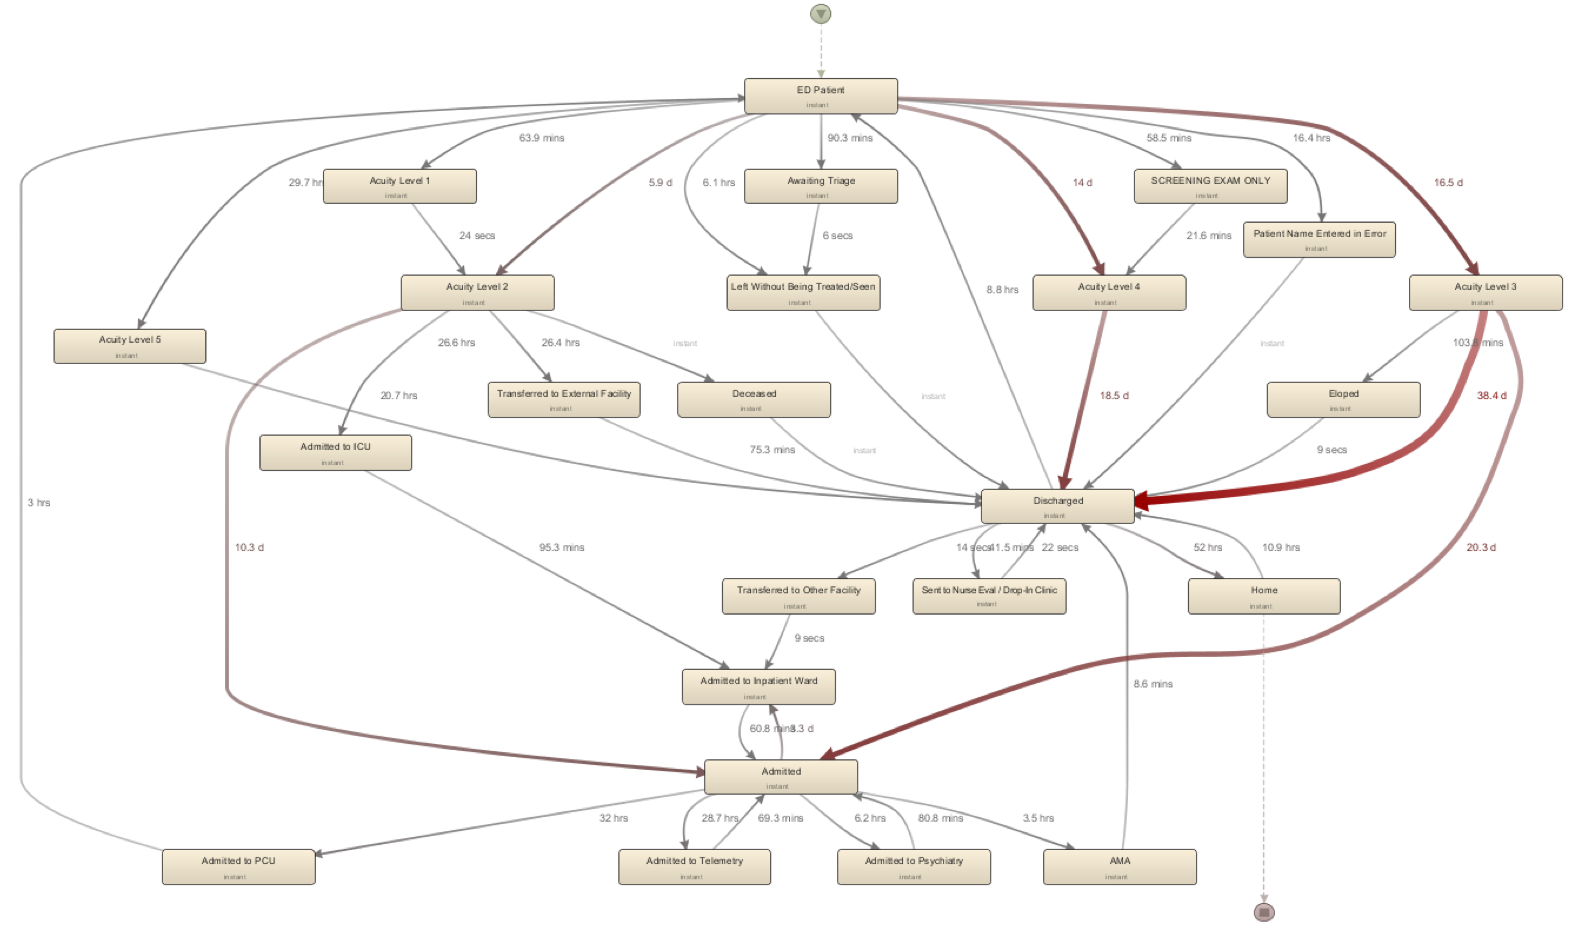
\includegraphics[width=0.8\linewidth]{img/ejemplo2.png}
%        \column{0.45\textwidth}
%          \pause[4]
%          \centering
%          
\includegraphics[width=0.5\linewidth]{img/homero_grita.jpg}
%
%          ¿Quién podría entender algo de un modelo como ese?
%      \end{columns}
%    \begin{itemize}
%        \item<5-> Para mejorar estos modelos se recurre a técnicas dentro del procesamiento de modelos
%                  llamadas de \textit{mejora de modelos}
%    \end{itemize}
%\end{frame}
                                           
\begin{frame}{Motivación}{Mejora de modelos}
  \begin{itemize}
    \item<2-> El problema con las técnicas de descubrimiento es que, en ocasiones, generan modelos
              demasiado complejos, conocidos como modelos \textit{spaghetti}.
  \end{itemize}
  \pause[3]
  \only<3>{
    \centering
    
\includegraphics[width=0.5\linewidth]{misc_images/lady_and_tramp.jpg}

    Los spaghetti pueden ser una muy buena idea para una cena romántica, 
    pero no son una buena idea para un modelo formal...
  }
  \begin{columns}
    \column{0.5\textwidth}
      \pause[4]
      \centering
      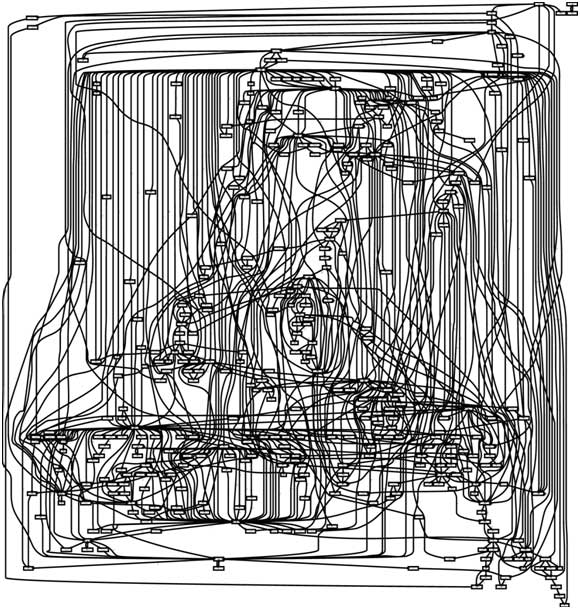
\includegraphics[width=0.8\linewidth]{img/spaghetti_model_2.jpg}
    \column{0.45\textwidth}
      \pause[5]
      \centering
      
\includegraphics[width=0.5\linewidth]{img/homero_grita.jpg}

      ¿Quién podría entender algo de un modelo como ese?
  \end{columns}
  \begin{itemize}
    \item<6-> Para mejorar estos modelos se recurre a técnicas dentro del procesamiento de modelos
              llamadas de \textit{mejora de modelos}
  \end{itemize}
\end{frame}

\begin{frame}{Motivación}{Mejora de modelos}
   \begin{itemize}
      \setlength\itemsep{0.4cm}
      \item<2-> Para aplicar las técnicas de mejora de modelos, utilizaremos información adicional a la
                obtenida de los logs de eventos.
      \item<3-> La información adicional puede consistir, por ejemplo, en la frecuencia con que ocurre cada traza, el 
          momento de ejecución, tiempo de duración de cada acción o bien de información
          acerca de las trazas que \textit{no} deben ocurrir.
    \end{itemize}
%    \pause[4]
%        Pero...¿qué es la información negativa?
%    \begin{itemize}
%      \item<5-> La información negativa consiste en un conjunto de trazas que el sistema no debe realizar nunca.
%    \end{itemize}
\end{frame}

\begin{frame}{Motivación}{Objetivo general}
  \centering
  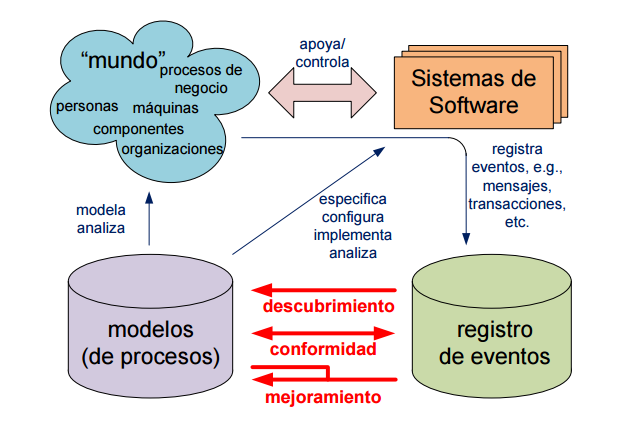
\includegraphics[width=0.95\linewidth]{img/pmcycle.png}
\end{frame}

\begin{frame}{Motivación}{Objetivo general}
  \begin{itemize}
    \setlength\itemsep{0.4cm}

    \item<1-> Obtener un modelo formal de manera automática a partir de los logs de eventos de un sistema.
    
    \item<2-> Optimizar el modelo obtenido mediante técnicas de mejora de modelos para obtener un modelo que
          resulte simple.
    
    \item<3-> Automatizar los puntos anteriores.

    \item<4-> Permitir la generación de mejoras a los procesos de los sistemas informáticos.
  
  \end{itemize}
\end{frame}

\section{Nociones preliminares}

\begin{frame}{Representación formal}{Redes de Petri}
    \begin{itemize}
      \setlength\itemsep{0.3cm}
      \item<2-> Existen diferentes representaciones formales utilizados en la minería de procesos.
                En particular, usaremos las \textbf{redes de Petri} como modelo de representación.
      \item<3-> Las redes de Petri fueron introducidas en el año 1962 por el matemático Carl Adam Petri
                para representar sistemas dinámicos con eventos concurrentes.
      \item<4-> Conforman un lenguaje gráfico y matemático con una semántica formal.
      \item<5-> Desde su creación han sido utilizadas, entre otros usos, para representación,
                análisis, verificación y simulación de sistemas de eventos discretos con 
                comportamiento dinámico.
    \end{itemize}
\end{frame}

\begin{frame}{Redes de Petri}{Definición formal}
  \begin{itemize}
    \item<2-> Formadas por dos componentes:
      \begin{itemize}
        \setlength\itemsep{0.2cm}
          \item<3-> Un grafo bipartito cuyos nodos se separan en los conjuntos disjuntos llamados
                    \textit{places} y \textit{transiciones} representa la red propiamente dicha.
          \item<4-> Un conjunto de fichas asignadas a los places de la red, denominado \textit{marking},
                    el cual es utilizado para simular el comportamiento dinámico y concurrente del sistema.
      \end{itemize}
  \end{itemize}

  \pause[5]

%  \begin{tcolorbox}[colback=gray!5!white,colframe=gray!50!black,
%  colbacktitle=gray!75!black,title=Red de Petri]
  \begin{block}{Redes de Petri}
    Formalmente, una red de Petri es una 4-upla $(P,T,F,M_0)$ donde:
     \begin{itemize}
        \item<6->{$P$ representa el conjunto finito de places.}
        \item<7->{$T$ representa el conjunto finito de transiciones.}
        \item<8->{La función \mbox{$F:(P \times T) \cup (T \times P)  \to \nat$} asigna el peso a los diferentes arcos.}
        \item<9->{Un marking inicial dado por la función \mbox{$M_0:P \to \nat$}.}
     \end{itemize}
  %\end{tcolorbox}
  \end{block}
\end{frame}

\begin{frame}{Redes de Petri}{Evolución}
    \begin{itemize}
      \setlength\itemsep{0.2cm}
      \item<2-> El dinamismo de una red viene dado por los markings, los cuales se van ``moviendo''
                de un place a otro tras la ejecución de las transiciones \emph{habilitadas}.
      \item<4-> Una transición $t$ se encuentra habilitada, en un marking $M$ si 
                contiene al menos tantas fichas en cada place que incide en $t$
                como marcan los arcos que los conectan:
                \bnnequation
                  \mbox{$\forall p \in P:~ M(p) \ge F(p,t) $}.
                \ennequation
      \item<5-> Ejecutar una transición $t$ sobre un place $p \in P$ en un cierto marking $M$ genera 
                un nuevo marking $M'$: \firing{M}{t}{M'}. 
      \item<6-> $M'$ viene definido de manera incremental como
                \bnnequation
                  M'(p) = M(p) - F(p,t) +  F(t,p)
                \ennequation
      %\item<2-> Dada una red de Petri $N$, se llama $\Language(N)$ al conjunto de secuencias de transiciones ejecutables sobre $N$.
      %\item<3-> Por su parte, al conjunto de markings alcanzable partiendo desde el marking inicial $M_0$,
      %          llamado \emph{conjunto alcanzable} de $N$, se lo nota $\rs(N)$.
  \end{itemize}
\end{frame}

\begin{frame}{Redes de Petri}{Ejemplo de la evolución de una red de Petri}
    \centering
    \only<1>{\usetikzlibrary{arrows,shapes,automata,petri,positioning}

\tikzset{
    placeyellow/.style={
        circle,
        thick,
        draw=yellow!75,
        fill=red!20,
        minimum size=6mm,
    },
    place/.style={
        circle,
        thick,
        draw=blue!75,
        fill=blue!20,
        minimum size=6mm,
    },
    transitionH/.style={
        rectangle,
        thick,
        fill=black,
        minimum width=8mm,
        inner ysep=2pt
    },
    transitionV/.style={
        rectangle,
        thick,
        fill=black,
        minimum height=8mm,
        inner xsep=2pt
    },
    transitionVgreen/.style={
        rectangle,
        thick,
        fill=green!25,
        minimum height=8mm,
        inner xsep=2pt
    },
    transitionVred/.style={
        rectangle,
        thick,
        fill=red!75,
        minimum height=8mm,
        inner xsep=2pt
    },
    transitionVdgreen/.style={
        rectangle,
        thick,
        fill=green!75,
        minimum height=8mm,
        inner xsep=2pt
    }
}


\begin{tikzpicture}[node distance=0.5cm and 1cm,>=stealth',bend angle=45,auto]
    \node [place,tokens=1,label=above:$P_1$] (p1) {};
    \node [transitionV,label=below:$T_1$] (t1) [right= of p1] {}
        edge[pre]   (p1);
    \node [place,tokens=1,label=above:$P_2$] (p2) [above right=of t1] {}
        edge[pre]   (t1);
    \node [place,tokens=2,label=above:$P_3$] (p3) [below right=of t1] {}
        edge[pre]   (t1);
    \node [transitionVred,label=below:$T_2$] (t2) [above right=of p3] {}
        edge[pre] node[swap]{\scriptsize 2} (p2)
        edge[pre]   (p3)
        edge[post,out=50,in=70,looseness=2,overlay]  (p1);
\end{tikzpicture}


}
    \only<2>{\usetikzlibrary{arrows,shapes,automata,petri,positioning}

\tikzset{
    placeyellow/.style={
        circle,
        thick,
        draw=yellow!75,
        fill=yellow!20,
        minimum size=6mm,
    },
    place/.style={
        circle,
        thick,
        draw=blue!75,
        fill=blue!20,
        minimum size=6mm,
    },
    transitionH/.style={
        rectangle,
        thick,
        fill=black,
        minimum width=8mm,
        inner ysep=2pt
    },
    transitionV/.style={
        rectangle,
        thick,
        fill=black,
        minimum height=8mm,
        inner xsep=2pt
    },
    transitionVgreen/.style={
        rectangle,
        thick,
        fill=green!25,
        minimum height=8mm,
        inner xsep=2pt
    },
    transitionVred/.style={
        rectangle,
        thick,
        fill=red!75,
        minimum height=8mm,
        inner xsep=2pt
    },
    transitionVdgreen/.style={
        rectangle,
        thick,
        fill=green!75,
        minimum height=8mm,
        inner xsep=2pt
    }
}


\begin{tikzpicture}[node distance=0.5cm and 1cm,>=stealth',bend angle=45,auto]
    \node [place,tokens=3,label=above:$P_1$] (p1) {};
    \node [transitionVdgreen,label=below:$T_1$] (t1) [right= of p1] {}
        edge[pre] node[swap]{\scriptsize 3}  (p1);
    \node [place,tokens=1,label=above:$P_2$] (p2) [above right=of t1] {}
        edge[pre]   (t1);
    \node [place,tokens=2,label=above:$P_3$] (p3) [below right=of t1] {}
        edge[pre]   (t1);
    \node [transitionVred,label=below:$T_2$] (t2) [above right=of p3] {}
        edge[pre] node[swap]{\scriptsize 2} (p2)
        edge[pre]   (p3)
        edge[post,out=50,in=70,looseness=2,overlay]  node[swap]{\scriptsize 4} (p1);
\end{tikzpicture}


}
    \only<3>{\usetikzlibrary{arrows,shapes,automata,petri,positioning}

\tikzset{
    placeyellow/.style={
        circle,
        thick,
        draw=yellow!75,
        fill=yellow!20,
        minimum size=6mm,
    },
    place/.style={
        circle,
        thick,
        draw=blue!75,
        fill=blue!20,
        minimum size=6mm,
    },
    transitionH/.style={
        rectangle,
        thick,
        fill=black,
        minimum width=8mm,
        inner ysep=2pt
    },
    transitionV/.style={
        rectangle,
        thick,
        fill=black,
        minimum height=8mm,
        inner xsep=2pt
    },
    transitionVgreen/.style={
        rectangle,
        thick,
        fill=green!25,
        minimum height=8mm,
        inner xsep=2pt
    },
    transitionVred/.style={
        rectangle,
        thick,
        fill=red!75,
        minimum height=8mm,
        inner xsep=2pt
    },
    transitionVdgreen/.style={
        rectangle,
        thick,
        fill=green!75,
        minimum height=8mm,
        inner xsep=2pt
    }
}


\begin{tikzpicture}[node distance=0.5cm and 1cm,>=stealth',bend angle=45,auto]
    \node [placeyellow,label=above:$P_1$] (p1) {};
    \node [transitionVdgreen,label=below:$T_1$] (t1) [right= of p1] {}
        edge[pre] node[swap]{\scriptsize 3}  (p1);
    \node [place,tokens=1,label=above:$P_2$] (p2) [above right=of t1] {}
        edge[pre]   (t1);
    \node [place,tokens=2,label=above:$P_3$] (p3) [below right=of t1] {}
        edge[pre]   (t1);
    \node [transitionVred,label=below:$T_2$] (t2) [above right=of p3] {}
        edge[pre] node[swap]{\scriptsize 2} (p2)
        edge[pre]   (p3)
        edge[post,out=50,in=70,looseness=2,overlay]  node[swap]{\scriptsize 4} (p1);
\end{tikzpicture}


}
    \only<4>{\usetikzlibrary{arrows,shapes,automata,petri,positioning}

\tikzset{
    placeyellow/.style={
        circle,
        thick,
        draw=yellow!75,
        fill=yellow!20,
        minimum size=6mm,
    },
    place/.style={
        circle,
        thick,
        draw=blue!75,
        fill=blue!20,
        minimum size=6mm,
    },
    transitionH/.style={
        rectangle,
        thick,
        fill=black,
        minimum width=8mm,
        inner ysep=2pt
    },
    transitionV/.style={
        rectangle,
        thick,
        fill=black,
        minimum height=8mm,
        inner xsep=2pt
    },
    transitionVgreen/.style={
        rectangle,
        thick,
        fill=green!60,
        minimum height=8mm,
        inner xsep=2pt
    },
    transitionVred/.style={
        rectangle,
        thick,
        fill=red!75,
        minimum height=8mm,
        inner xsep=2pt
    },
    transitionVdgreen/.style={
        rectangle,
        thick,
        fill=green!75,
        minimum height=8mm,
        inner xsep=2pt
    }
}


\begin{tikzpicture}[node distance=0.5cm and 1cm,>=stealth',bend angle=45,auto]
    \node [place,label=above:$P_1$] (p1) {};
    \node [transitionVdgreen,label=below:$T_1$] (t1) [right= of p1] {}
        edge[pre] node[swap]{\scriptsize 3}  (p1);
    \node [placeyellow,tokens=2,label=above:$P_2$] (p2) [above right=of t1] {}
        edge[pre]   (t1);
    \node [placeyellow,tokens=3,label=above:$P_3$] (p3) [below right=of t1] {}
        edge[pre]   (t1);
    \node [transitionVred,label=below:$T_2$] (t2) [above right=of p3] {}
        edge[pre] node[swap]{\scriptsize 2} (p2)
        edge[pre]   (p3)
        edge[post,out=50,in=70,looseness=2,overlay]  node[swap]{\scriptsize 4} (p1);
\end{tikzpicture}


}
    \only<5>{\usetikzlibrary{arrows,shapes,automata,petri,positioning}

\tikzset{
    placered/.style={
        circle,
        thick,
        draw=red!75,
        fill=red!20,
        minimum size=6mm,
    },
    place/.style={
        circle,
        thick,
        draw=blue!75,
        fill=blue!20,
        minimum size=6mm,
    },
    transitionH/.style={
        rectangle,
        thick,
        fill=black,
        minimum width=8mm,
        inner ysep=2pt
    },
    transitionV/.style={
        rectangle,
        thick,
        fill=black,
        minimum height=8mm,
        inner xsep=2pt
    },
    transitionVgreen/.style={
        rectangle,
        thick,
        fill=green!60,
        minimum height=8mm,
        inner xsep=2pt
    },
    transitionVred/.style={
        rectangle,
        thick,
        fill=red!75,
        minimum height=8mm,
        inner xsep=2pt
    },
    transitionVdgreen/.style={
        rectangle,
        thick,
        fill=green!75,
        minimum height=8mm,
        inner xsep=2pt
    }
}


\begin{tikzpicture}[node distance=0.5cm and 1cm,>=stealth',bend angle=45,auto]
    \node [place,label=above:$P_1$] (p1) {};
    \node [transitionVred,label=below:$T_1$] (t1) [right= of p1] {}
        edge[pre] node[swap]{\scriptsize 3}  (p1);
    \node [place,tokens=2,label=above:$P_2$] (p2) [above right=of t1] {}
        edge[pre]   (t1);
    \node [place,tokens=3,label=above:$P_3$] (p3) [below right=of t1] {}
        edge[pre]   (t1);
    \node [transitionV,label=below:$T_2$] (t2) [above right=of p3] {}
        edge[pre] node[swap]{\scriptsize 2} (p2)
        edge[pre]   (p3)
        edge[post,out=50,in=70,looseness=2,overlay]  node[swap]{\scriptsize 4} (p1);
\end{tikzpicture}


}
\end{frame}

\begin{frame}{Logs de eventos}{Definición}
  \begin{itemize}
    \setlength\itemsep{0.2cm}
    \item<2-> Un \textit{evento} refiere a la ocurrencia de una actividad de un sistema $\sys$.
    \item<3-> Una \textit{traza} de eventos se define como una sucesión ordenada de eventos.
    \item<4-> Un \textit{log de eventos} corresponde a un conjunto de trazas correspondientes 
              a una instancia única de ejecución de $\sys$ y se conforma de:
              \begin{itemize}
                  \item Un conjunto de actividades.
                  \item Un cierto orden temporal de ocurrencia.
                  \item Una etiqueta que diferencia las diferentes instancia en trazas
              \end{itemize}
    \item<5-> Además, un log puede contener datos adicionales que, aunque no sean fundamentales, pueden
ayudar a la minería de procesos otorgándole mayor nivel de detalle y claridad.
  \end{itemize}
\end{frame}






%\section{Conclusión y trabajos futuros}
%\begin{frame}{Conclusión}{}
%
%Conclusiones:
%\begin{itemize}
%  \item Pudimos desarrollar una solución para la generación automática de descripciones en lenguaje natural para clases de prueba generadas por el TTF.
%
%  \item La solución propuesta es independiente del dominio de aplicación y del número de operaciones del sistema.
%
%  \item Implementamos exitosamente un prototipo que fue integrado a las funcionalidades de Fastest.
%\end{itemize}    
%\end{frame}
%
%\begin{frame}{Trabajo futuro}{}
%Trabajos futuros:
%\begin{itemize}
%  \item Evaluación de textos generados por el sistema realizado (en términos de exactitud, fluidez, etc.).
%
%  \item Ampliar la totalidad de operadores aceptados por el sistema.
%
%  \item Profundizar el trabajo sobre los datos de entrada agregando más tareas de razonamiento con los datos.
%
%  \item Expandir el sistema para que sea capaz de producir descripciones en otros idiomas.
%\end{itemize}                         
%\end{frame}
%                                
\frame{\begin{center}
\textbf{¿Preguntas?}
\end{center}}

\frame{\begin{center}
\textbf{¡Gracias!}
\end{center}}
               
                                                                                      
\end{document} 
